\documentclass[12pt, fleqn]{article}
\usepackage{../../../template/template}

%сам документ
\begin{document}
\begin{center}
  \huge Практика по матану, 3 сем
  
  \Large (преподаватель Роткевич А. С.)
  
  \large Записал Костин П.А.
\end{center}

Данный документ неидеальный, прошу сообщать о найденных недочетах в \href{https://vk.com/drab_existence_a}{вконтакте}
\tableofcontents
\newpage

%билеты
\section{Функции от нескольких переменных}
\subsection{02.09.2019}
\subsubsection{Основные определения}

\begin{definition}
    $\rho: X * X \ra \R$ - метрика, если
    \begin{enumerate}                               
    	\item $\rho(x,y) \geqslant 0$, $\rho(x,y)=0 \Lra x=y$
    	\item $\rho(x,y)=\rho(y,x)$
    	\item $\rho(x,y) \leqslant \rho(x,z)+\rho(z,y)$
    	
    	$(X,\rho)$ - метрическое пространство
	\end{enumerate} 
\end{definition}

\begin{examples}
    \begin{enumerate}  
        \item $\R$ $\rho(x,y)=|x-y|$
        \item $x \neq \varnothing$ $\rho(x,y)=
            \begin{cases}
                1, \q x \neq y\\
                0, \q x=y
            \end{cases}$
        \item $\R^n$, $n \geqslant 1$ $\rho(x,y)=\sqrt{(x_1-y_1)^2+...+(x_n-y_n)^2}$,
        
        где $x=(x_1,...,x_n)$ $y=(y_1,...,y_n)$
    \end{enumerate} 
\end{examples}

\begin{definition}
    $\rho_1, \rho_2: X*X \ra \R$ - метрики, тогда $\rho_1, \rho_2$ - эквивалентны, если 
    
    (они задают одну топологию) $c_1 \rho_1 (x,y) \leqslant \rho_2 (x,y) \leqslant c_2 \rho_1(x,y)$ для $c_1,c_2>0$ - $\const$
\end{definition}

\begin{example}
    $\R^2$ $\rho_1(x,y) = \sqrt{(x_1-y_1)^2 + (x_2-y_2)^2} \leqslant \sqrt{2 \rho_2^2(x,y)}$
    
    $\rho_2(x,y)=max(|x_1-y_1|, |x_2-y_2|)$ (упр.)
    
    $\frac{1}{\sqrt{2}} \rho_1(x,y) \leqslant \rho_2(x,y) \leqslant \rho_1(x,y)$
    
    Пусть $\rho_3(x,y)=(|x_1-y_1|^p+...|x-n-y_n|^p)^{\frac{1}{p}}$, $p \geqslant 1$
    
    Если $p \ra \infty$ $\rho_3 \ra \rho_2$
    
    $l_n^p=(\R^n,\rho_3)$ - пространство Лебега конечномерное
    
    (упр.) Д-ть, что все метрики эквивалентны $(\rho_1,\rho_2,\rho_3)$
    
    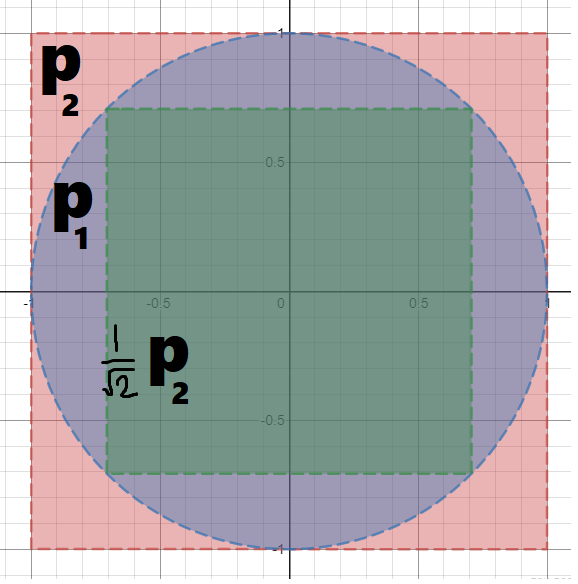
\includegraphics[scale=0.3]{pics/p1p2p3.png}
\end{example}

\begin{definition}
    $\rho: X*X \ra \R$ - метрика, 
    
    Открытым шаром в X относительно метрики $\rho$ называется мн-во $B_r(x)=B(x,r)=\{y \in X: \rho(x,y) < r \}$
    
    Замкнутым шаром называется $\ol{B}_r(x)=\{y \in X: \rho(y,x) \leqslant r \}$
    
    Сферой называется $S_r(x)=\{y \in X: \rho(x,y)=r \}$
\end{definition}

\begin{upr}
    Замкнутый шар - не всегда замыкание шара (см. дискретную метрику)
\end{upr}

\begin{example}
    $l^p=\{ \{x_n\}_{n=1}^\infty: \sum\limits_{n=1}^\infty |x_n|^p < \infty \}$ $1 \leqslant p < \infty$
    
    $\rho(\{x_n\}_{n=1}^\infty, \{y_n\}_{n=1}^\infty) = (\sum\limits_{n=1}^\infty (x_n-y_n)^p)^{\frac{1}{p}}$
    
    $l^p$ - пр-во Лебега (последовательностей)
\end{example}

\begin{example}
    $C[0,1]$ - пр-во непр. функций
    
    $\rho(f,g)=\max\limits_{[0,1]} |f-g|$ - полна (любая фундаментальная последовательность сходится)
    
    $\rho_p(f,g)=(\int\limits_0^1 |f-g|^p dx)^{\frac{1}{p}}$ - не полная
\end{example}

\begin{definition}
    $(X, \rho)$ - метр. пр-во, $\{x_k\}_{k=1}^\infty \subset X$, $a \in X$ $x_k \ra a$ в пр-ве X по метрике $\rho$, если $\rho(x_n,a) \us{k \ra \infty}{\ra} 0$
\end{definition}

\begin{examples}
    $\R^2$ $M_k=(x_k, y_k)$ $P=(a,b)$ $M_k \ra P$ в евкл. метрике, т.е. $\rho(M_k,P)=\sqrt{(x_k-a)^2+(y_k-b)^2} \us{k \ra \infty}{\ra} 0 \Lra x_k \ra a,\ y_k \ra b$
\end{examples}

\begin{remark}
    Есть $\rho_1,\rho_2$ - экв. метрики, то $\rho_1(x_k,a) \ra 0 \Lra \rho_2(x_k,a) \ra 0$
\end{remark}

\begin{upr}
    $x_k \ra a,\ x_k \ra b \Ra a=b$
    
    ($\rho(a,b) \leqslant \rho(a, x_k) + \rho(x_k,b) \ra 0 \Ra \rho (a,b) \ra 0 \Ra a=b$)
\end{upr}

\begin{definition}
    $E \subset X$, $(X, \rho)$ - метр. пр-во, то $a \in X$ - т. сгущ. E, если 
    
    $\forall \E \ \e x \in E: \rho(a,x) < \E$
\end{definition}

\begin{definition}
    $f:E \ra Y$ $(X, \rho)$, $(Y,d)$ - метр. пр-ва $(E \subset X)$, а - т. сгущ. E, $A \in Y$, 
    
    тогда A - предел отображения f в точке а, если 
    
    $f(x) \ra A$ при $x \in E \setminus \{a\}\ra a$\\
    (или $\forall \E>0 \q \e \delta>0: \rho(x,a)<\delta$ и $x \in E \subset \{a\}$, то $d(f(x),A) < \E)$\\
    Обозначение: $A=\lim\limits_{x \ra a} f(x)$ или $f(x) \ra A$ $x \ra a$
\end{definition}

\begin{remark}
    $A=\lim\limits_{x \ra a} f(x) \Lra \forall \E > 0 \ \e \delta>0: f(B_\delta(a) \setminus \{a\}) \subset B_\E (A)$
\end{remark}

\newpage
\subsection{05.09.2019}
\subsubsection{Примеры для $\R^2$}

Будем в $\R^2$, $\rho((x_1,y_1), (x_2,y_2)) = \sqrt{(x_1-x_2)^2 + (y_1-y_2)^2}$
\begin{definition}
    $f: E \ra \R$, $E \subset \R^2$, $a \in \R^2$ - точка сгущения, $\lim\limits_{x \ra a} f(x) = F$, если 
    
    $\forall \E>0 \q \e \delta>0: 0<\rho(x,a)<\delta$, $x \in E \Ra |f(x)-A|<\E$ 
\end{definition}
В $\R^2$ работают: 

арифм. действия, теор. о двух миллиционерах, критерий Коши:
\begin{definition}
    $f: E \ra \R$, частный случай $\e \lim\limits_{x \ra a} f \Lra \forall \E>0 \q \e \delta > 0:$
    
    $|f(x)-f(y)|<\E$ $0<\rho(x,a), \rho(y,a)<\delta$ (упр)
\end{definition}

\begin{upr}
    $\e \lim\limits_{x \ra a} f \Lra \forall \{x_n\}: x_n \neq a \q x_n \ra a$ ($\rho(x_n,a) \ra 0$) $\e \lim\limits_{n \ra \infty} f(x_n)$
\end{upr}

Обозначение: $\us{y \ra y_0}{\lim\limits_{x \ra x_0}} f(x,y) = \lim\limits_{(x,y) \ra (x_0,y_0)} f(x,y)$ - предел функции в т. $(x_0,y_0)$

\begin{example}
    $f(x,y)=(x+y)\sin \frac{1}{x} \sin \frac{1}{y}$, $\us{y \ra 0}{\lim\limits_{x \ra 0}} f(x,y) = 0$, т.к.$|f(x,y)| \leqslant |x|+|y| \us{y \ra 0}{\us{x \ra 0}{\ra}} 0$, $\not \e \lim\limits_{y \ra 0} \lim\limits_{x \ra y} f(x,y)$
\end{example}

\begin{example}\\
    $f(x,y)=\frac{x^2 y^2}{x^2 y^2 + (x-y)^2}$ - не существует, так как $\lim f(x,x)=1$, $f(x,2x)=0$
\end{example}

\begin{example}
    Построить $f(x,y)$ т.ч. $\forall a,b$ $\e \lim\limits_{t \ra 0} f(at,bt)=A$, но $\not \e \us{y \ra 0}{\lim\limits_{x \ra 0}} f(x,y)$
    
    $f=\frac{y^2}{x}=\frac{b^2}{a} t \ra 0$, но при $x=\frac{1}{n^2}$, $y=\frac{1}{n}$ предел - единица
\end{example}

\begin{remark}
    Если $\upgamma(t) \us{t \ra t_0}{a} \in \R^2$ и $\e \lim\limits_{x \ra a} f(x)=A$, то $\e \lim\limits_{t \ra t_0} f(\upgamma(t))$
\end{remark}

\begin{remark}
    Если $\forall \upgamma: \upgamma(t) \ra a \in \R^2$ и $\e \lim f(\upgamma(t))$, то $\e \lim\limits_{x \ra a} f$
\end{remark}

\begin{remark}
    $\lim\limits_{x \ra x_0} \lim\limits_{y \ra y_0} f(x,y)$ - не предел по кривой (из-за необязательного равенства предела и значения в пределе). Более формально: пусть $=\lim\limits_{x \ra x_0} \ol{f}(x)$
    
    $\ol{f}(x)=\lim\limits_{y \ra y_0} f(x,y) \neq$(не обязательно) $\neq f(x,y_0)$
\end{remark}

\begin{definition}\\
    $\us{y \ra +\infty}{\lim\limits_{x \ra +\infty}} f(x,y)=A$, если 
    
    $\forall \E>0 \ \e M>0: \forall x,y: \max(x,y)>M \ |f(x,y)-A|<\E$
\end{definition}

\begin{example}\\
    $f=\frac{y}{x} tg(\frac{x}{x+y})$ - не имеет предела, $f(x,x)=tg(\frac{1}{2})$, $f(x,x^2)=x tg(\frac{1}{1+x}) \ra 0$
\end{example}

\newpage
\subsection{09.09.2019}
\subsubsection{Ещё больше определений}
\begin{definition}
\begin{enumerate}
        \item $A=\us{y \ra +\infty}{\lim\limits_{x \ra +\infty}} f(x,y)$, если 
        
        $\forall \E>0 \ \e M>0: x>M \ y>M \Ra |f(x,y)-A| < \E$
        \item $A=\us{y \ra +\infty}{\lim\limits_{x \ra +\infty}} f(x,y)$, если 
        
        $\forall \E>0 \ \e M>0: |x|>M \ |y|>M \Ra |f(x,y)-A| < \E$
        \item $A=\lim\limits_{P \ra \infty} f(P) \ P \in \R^2$, если 
        
        $\forall \E>0 \ \e M>0: \rho(0, P)>M \Ra |f(x,y)-A| < \E$
    \end{enumerate}
\end{definition}

\begin{remark}
    Демидович по первым двум определениям
\end{remark}

\begin{definition}
    Для конечного предела: $A=\lim\limits_{x \ra a \  y \ra +\infty} f(x,y)$, если 
    
    $\forall \E>0 \q \e M>0 \q \delta > 0: y>M \q |x-a| < \delta \Ra |f(x,y)-A| < \E$
\end{definition}

\subsubsection{Ещё больше примеров}

\begin{example}
    $\us{y \ra +\infty}{\lim\limits_{x \ra +\infty}} (\dfrac{x y}{x^2+y^2})^{x^2}$
\end{example}

\begin{sol}
    Заметим, что $\dfrac{x y}{x^2+y^2} \leqslant \dfrac{1}{2} \Ra 2xy \leqslant x^2 + y^2 \Ra 0 \leqslant (x-y)^2\text{ для x }\neq y$
    \\
    Значит дробь стремится к 0
\end{sol}

\begin{example}
    $\us{y \ra 0}{\lim\limits_{x \ra 0}} (\dfrac{x y}{x^2+y^2})^{x^2}$
\end{example}

\begin{sol}
    При $x=y$ предел $\dfrac{1}{2}$\\
    При $x=y^2$ предел 0
\end{sol}

\begin{example}
    $f=\sin(\dfrac{\pi y^2}{x^2 + 3y^2})$\\
    Найти $\us{y \ra +\infty}{\lim\limits_{x \ra +\infty}} f$, $\lim\limits_{x \ra \infty} \lim\limits_{y \ra \infty} f$, $\lim\limits_{y \ra \infty} \lim\limits_{x \ra \infty} f$
\end{example}

\begin{sol}
    Первый не имеет предела ($x=y$, $x=\sqrt{y})$. Второй $\dfrac{\sqrt{3}}{2}$. Третий 0
\end{sol}

\begin{example}
    $\us{y \ra +\infty}{\lim\limits_{x \ra +\infty}} \dfrac{sin(y-x^2)}{y-x^2}$
\end{example}

\begin{sol}
    $z=y-x^2$, $z \ra 0 \Ra x,y \ra 0$
    
    $|z| \leqslant |x| + |y| \leqslant 2 \sqrt{x^2+y^2}$
\end{sol}

\begin{example}
    $f=\dfrac{1-\sqrt[3]{sin^4 x + cos^4 y}}{\sqrt{x^2+y^2}}$, найти $\us{y \ra 0}{\lim\limits_{x \ra 0}} f$
\end{example}

\begin{sol}
    $1-\sqrt[3]{t} \us{t \ra 1}{~} \dfrac{1-t}{3}$ (т.к. $1-\sqrt[3]{t}=\frac{1-t}{1+\sqrt[5]{t}+\sqrt[3]{t^2}}$)
    
    Значит $\us{y \ra 0}{\lim\limits_{x \ra 0}} f = \us{y \ra 0}{\lim\limits_{x \ra 0}} \frac{1}{3} \dfrac{1-(sin^4 x + cos^4 y)}{\sqrt{x^2+y^2}} = \us{y \ra 0}{\lim\limits_{x \ra 0}} \dfrac{2sin^2 y - sin^4 y - sin^4 x}{3 \sqrt{x^2+y^2}}$
    
    Заменим по Тейлору: $=\us{y \ra 0}{\lim\limits_{x \ra 0}} \dfrac{2y^2 + \ol{o}(y^3)-x^4 + \ol{o}(x^6)}{3 \sqrt{x^2+y^2}}$
    
    Попробуем оценить по модулю $|\dfrac{2y^2-x^4}{\sqrt{x^2+y^2}}|$, заметим что $y^2 \leqslant x^2 + y^2$, 
    
    $x^4 \leqslant 2(x^2+y^2) \leqslant x^2+y^2$ (для $x^2+y^2 < 1)$, 
    
    чтобы избавиться от $\ol{o}$ оценим так: 
    
    $\ol{o} + y^2 \leqslant 2(x^2 + y^2)$, $\ol{o} + x^4 \leqslant 2(x^2+y^2) \leqslant x^2+y^2$
    
    Тогда $|\dfrac{2y^2-x^4}{\sqrt{x^2+y^2}}| \leqslant 2 \dfrac{3(x^2+y^2)}{\sqrt{x^2+y^2}} \leqslant 6 \sqrt{x^2+y^2} \ra 0$
\end{sol}

\newpage
\subsection{12.09.2019}
\subsubsection{Некоторые особенные примеры}
\begin{example}
    $\us{y \ra 1}{\lim\limits_{x \ra 0}} (1+x)^{\frac{1}{x+x^2 y}}=\us{y \ra 1}{\lim\limits_{x \ra 0}} ((1+x)^{\frac{1}{x}})^{\frac{1}{1+x y}}=e$
\end{example}

\begin{example}
    $f(x,y)=\begin{cases} \frac{x^3-xy^2}{x^2+y^2} &,x^2+2^2 \neq 0\\ a & , else \end{cases}$\\
    1) $a=?$, т.ч. f - непр\\
    2) $a=?$, f - непрю на прямых, проходящих через 0\\
\end{example}

\begin{sol}
    1) $a=\us{y \ra 0}{\lim\limits_{x \ra 0}} \frac{x^3-x y^2}{x^2+y^2}=\us{y \ra 0}{\lim\limits_{x \ra 0}} x \frac{x^2-y^2}{x^2+y^2}=0$
\end{sol}

\begin{remark}
    $x^n y^m \leqslant (\sqrt{x^2+y^2})^{n+m}$ и $|x| \leqslant \sqrt{x^2+y^2}$
\end{remark}

\subsubsection{Частные производные. Определения}
$f: \Omega \subset \R^3 \ra \R$, $P_0=(x_0,y_0,z_0)$
\begin{definition}
    f - диф. в точке $P_0$, если $\e A,B,C \in \R$, т.ч.\\
    $f(x_0,+\delta x, y_0 + \delta y, z+\delta z =f(x_0,y_0,z_0)+A \delta x+ B \delta y + C \delta z+\ol{o} (\sqrt{(\delta x)^2+(\delta y)^2+ (\delta z)^2})$\\
    Пусть $h=(\delta x, \delta y, \delta z)^T$\\
    $f(P_0+h)=f(P_0)=\begin{pmatrix} A\\ B\\ C \end{pmatrix}^T h + \ol{o}(|h|)$\\
    $df(x,y,z)=A dx+B dy+C dz$\\
    Дифференциал сопоставляет $(dx, dy, dz) \ra A dx+B dy+C dz$ 
\end{definition}

\begin{definition}
    Частной произв. по перем. x в т. $(x_0,y_0,z_0)$ называется предел (если $\e$)
    \[\lim\limits_{t \ra 0} \frac{f(x_0+t,y_0,t_0)-f(x_0,y_0,z_0)}{t}=\frac{\d f}{\d x}(x_0,y_0,z_0)=f'_x(x_0,y_0,z_0)\]
\end{definition}

\subsubsection{Частные производные. Примеры}
\begin{utv}
    f - дифф. $\Ra$ $\e$ част. пр. и $A= \frac{\d f}{\d x} (x_0,y_0,z_0)$, $B=\frac{\d f}{\d x}$, $C=\frac{\d f}{\d x}$
\end{utv}

Производные старшего порядка \[\frac{\d^2 f}{\d x^2} = \frac{\d}{\d x} (\frac{\d f}{\d x})\]
\[\frac{\d^2 f}{\d x \d y}= \frac{\d}{\d x} \frac{\d f}{\d y} \neq \text{(не всегда) }\frac{\d}{\d y} (\frac{\d f}{\d x}) = \frac{\d^2 f}{\d y \d x}\]

Частные производные сложной функции 
\[w=f(x,y,z),\ \R^2 \ra \R^3.\ (u,v) \ra(\varphi(u,v), \psi(u,v), \chi(u,v))\]
\[w=f(\varphi(u,v), \psi(u,v), \chi(u,v))\]
\[\frac{\d w}{\d u}=\frac{\d f}{\d x}, \frac{\d \varphi}{\d u}+ \frac{\d f}{\d y} \frac{\d \psi}{\d u}+\frac{\d f}{\d z} \frac{\d \chi}{\d u}\]
\[\frac{\d w}{\d v}=\frac{\d f}{\d x} \frac{\d \varphi}{\d v}+\frac{\d f}{\d y} \frac{\d \psi}{\d v}+ \frac{\d f}{\d z} \frac{\d \chi}{\d v}\]
\[
\begin{pmatrix}
\frac{\d w}{\d u}\\
\frac{\d w}{\d v}
\end{pmatrix}=
\begin{pmatrix}
\frac{\d \varphi}{\d u} & \frac{\d \psi}{\d u} & \frac{\d \chi}{\d u}\\
\frac{\d \varphi}{\d v} & \frac{\d \psi}{\d v} & \frac{\d \chi}{\d v}
\end{pmatrix}
\begin{pmatrix}
\frac{\d f}{\d x}\\
\frac{\d f}{\d y}\\
\frac{\d f}{\d z}
\end{pmatrix}
\]

\begin{example}
    \[\frac{\d^2 w}{\d u \d v} = \frac{\d f}{\d x} \frac{\d^2 \varphi}{\d u \d v}+(\frac{\d^2 f}{\d x^2} \frac{\d u}{\d v}+\frac{\d^2 f}{\d x \d y} \frac{\d \psi}{\d v}+\frac{\d^2 f}{\d x \d z} \frac{\d \chi}{\d v}) \frac{\d \varphi}{\d u}+...\]
\end{example}

\begin{example}
    \[F=f(x,x y, x y z)=f(u,v,w)\]
    \[\frac{\d F}{\d x}=\frac{\d f}{\d u} 1+ \frac{\d f}{\d v} y + \frac{\d f}{\d w} yz\]
    \[\frac{\d}{\d x}=\frac{\d}{\d u}+y \frac{\d}{\d v}+uz \frac{\d}{\d w}\]
    \[\frac{\d^2 F}{\d x^2} = \frac{\d}{\d x}(\frac{\d f}{\d u})+ \frac{\d}{\d x}(\frac{\d f}{\d v}) y + \us{=0}{\frac{\d f}{\d v} \frac{\d}{\d x} (y)}+ \frac{\d}{\d x} (\frac{\d f}{\d w}) yz + \frac{\d f}{\d w} \frac{\d}{\d x} (yz)\]
    \begin{multline*}
        \frac{\d}{\d x} (\frac{\d f}{\d u})=\frac{\d^2 f}{\d u^2}+ y \frac{\d^2 f}{\d u \d v}+yz \frac{\d^2 f}{\d u \d w} =\\ = \frac{\d^2 f}{\d u^2}+y \frac{\d^2 f}{\d v^2}+(yz)^2 \frac{\d^2 f}{\d w^2}+z y \frac{\d^2 f}{\d u \d v} + 2y^2 z \frac{\d^2 f}{\d v \d w} + 2yz \frac{\d^2 f}{\d u \d w}
    \end{multline*}
    
\end{example}

\begin{example}
    Дано $u=x^y$, найти $\dfrac{\d^2 u}{\d x^2}$, $\dfrac{\d^2 u}{\d y^2}$, $\dfrac{\d^2 u}{\d x \d y}$
    \\
    \[\dfrac{\d u}{\d x}=y x^{y-1}, \q \dfrac{d^2 u}{\d x^2}=y(y-1)x^{y-2}\]
    \[\dfrac{\d u}{\d y}=\ln(x) x^y, \q \dfrac{\d^2 y}{\d y^2}=\ln^2(x) x^y\]
    \[\dfrac{\d^2 u}{\d x \d y}=x^{y-1}+y \ln(x) x^{y-1}\]
\end{example}

\end{document}